% !TEX root = ../../thesis.tex

\newpage
\thispagestyle{plain}
\mbox{}
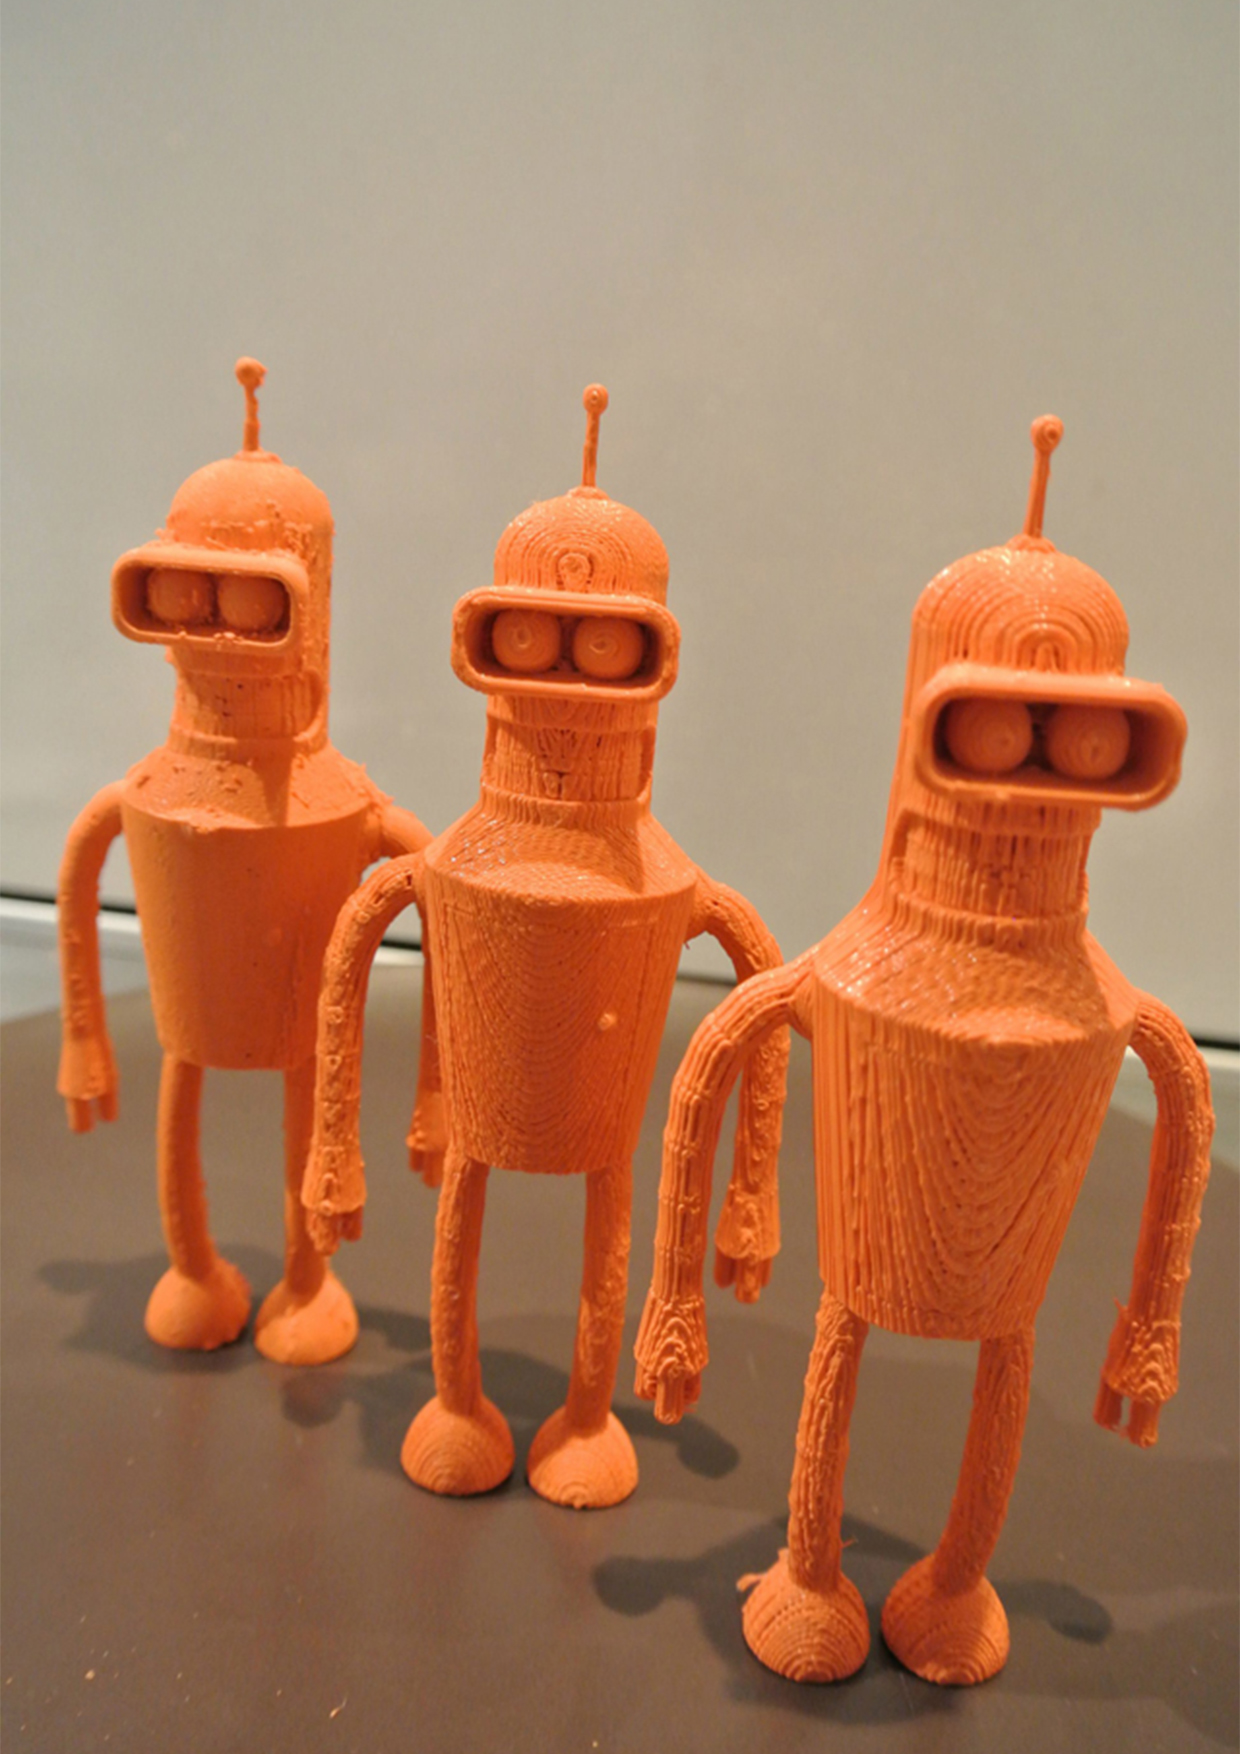
\includepdf{/Users/matthieulapeyre/Documents/phd_thesis/media/3DprintedBlender.pdf}
\chapter{The open hardware and 3D printing revolution} % (fold)



\section{Introduction} % (fold)

The last decades, thanks to the democratization of personal computers and the development of Internet, computer science has known a great expansion.  Open source software played a major role in this expansion. Indeed, most of the web sever are running under open source operating system (Linux) while open source software ...
While copying bits of a software is virtually free, producing the atoms of a hardware has a cost.
Meanwhile the production of both mechanic or electronics hardware components  was limited to two options. Either it was handcrafted or mass produced. Indeed
production in small or medium series are extremely difficult to achieve.
Conventional manufacturing processes require the production of specific tools, the programming of complex machine, the human intervention to put the part along the different tool etc ...
Mosts of the cost are in the up-front tooling, and the more complicated a product is, the more it costs. Thus, most of companies will not accept to run a whole production process just for few units and if they accept the cost will be so high than most prototypes never find a way to reach people outside the workshop they had been created. Only big companies were able to raise enough money to produce new hardware and the niche products and personalization were left aside.

These limitations are going to change. First, new economical model are raising based on crowd-funding allowing inventor to get the fundings needed to make their idea produced.

standardisation

consomery goods

But the rules are currently changing. Rapid prototyping is under democratization ans give access to a Low Cost production to everyone.
It is the makers revolution which is predicted to deeply change the economical model of things.
The early adopter of this new tools are called "makers".

This will lead to the emergence of small batch product and variability. From variabilty come the innovation (Pick) and


Need:

Problems associated to hardware diffusion are not specific to commercial products. In scientific research and especially in the robotics field, the production of prototype is a major issue. The same production problem occur.

While

These problems occuring in the inventor/entrepreneur world are also the case in research.

The same problem occurs in the research community. We produce prototype, we need to explore design we do not know how it will works because it is under research.
Acroban was a perfect example, some very good idea such as a multi-articulated column but a realisation handcrafted leading to an impossibility to share our research.

In this chapter, we will discuss the emergence of new production tools also coming with new user behavior under the DIY, makers and open

While open source software project contributed to some major innovation in the building of internet. The open hardware was limited by its

Open source had a major role on the software innovation.

Open soft a montré des choses.
Open hardware est un vieu truc mais qui reste limité
arrivé de method de RP efficace et low cost
Arrivée d'arduino

de plus en plus de tools open source pour créer de nouveaux tools.


The open hardware and 3D printing revolution ( arduino, les imprimantes 3D, les fablabs, de nouvelles façons de créer/produire)

\section{Open source hardware} % (fold)

\subsection{History} % (fold)
- Machine à soie de Lyon.

- Homebrew computing club
% ref( http://en.wikipedia.org/wiki/Homebrew_Computer_Club, http://www.atariarchives.org/deli/homebrew_and_how_the_apple.php)


\subsubsection{Open Hardware definition} % (fold)

\begin{figure}[]
    \begin{center}
        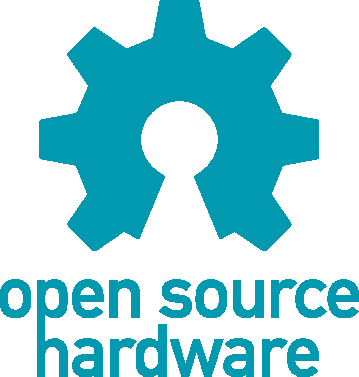
\includegraphics[height=5cm]{oshw-logo.pdf}
    \end{center}
    \caption{The open source hardware logo}
    \label{fig:ohw-logo}
\end{figure}

\begin{quotation}
  \emph{Open source hardware is hardware whose design is made publicly available so that anyone can study, modify, distribute, make, and sell the design or hardware based on that design. The hardware’s source, the design from which it is made, is available in the preferred format for making modifications to it. Ideally, open source hardware uses readily-available components and materials, standard processes, open infrastructure, unrestricted content, and open-source design tools to maximize the ability of individuals to make and use hardware. Open source hardware gives people the freedom to control their technology while sharing knowledge and encouraging commerce through the open exchange of designs.}

  -- \textbf{Open Source Hardware Association (OSHW)}
\end{quotation}


\subsection{Open source licenses for hardware} % (fold)



Apache, MIT License, GPL, BSD
\subsubsection{Creative Commons licenses} % (fold)



http://creativecommons.org/about/downloads
\begin{NFfigure}
    \begin{center}
        
\includegraphics[height=2cm]{cc-logo.pdf}
    \end{center}
    \caption{Creative Commons logo}
    \label{fig:cc-logo}
\end{NFfigure}

The Creative Commons licenses are based on four major condition modules:
\begin{description}
    \item[BY] Attribution: requiring attribution to the original author.
    \item[NC] Non Commercial: requiring the work is not used for commercial purposes
    \item[ND] No Derivative works: allowing only the original work, without derivatives
    \item[SA] Share Alike: allowing derivative works under the same or a similar license (later or jurisdiction version).
\end{description}


The combination of these modules leads to six licenses.

\begin{description}
    \item[] 
\includegraphics[width=2.5cm]{cc-by.pdf} \\ \textbf{Attribution CC BY} People can distribute, remix, tweak and build upon the licensed work, even commercially, as long as they credit the authors of the original creation.
    \item[Attribution-ShareAlike CC BY-SA] \begin{center} 
\includegraphics[width=2.5cm]{cc-by-sa.pdf} \end{center} People can distribute, remix, tweak and build upon the licensed work, even commercially, as long as they credit the authors and license their new creations under the identical terms. \textbf{This license is often compared to “copyleft” free and open source software licenses.}
    \item[Attribution-NoDerivs CC BY-ND] \begin{center} 
\includegraphics[width=2.5cm]{cc-by-nd.pdf} \end{center} This license allows for redistribution, commercial and non-commercial, as long as it is passed along unchanged and in whole, with credit to the authors.
    \item[Attribution-NonCommercial CC BY-NC] \begin{center} 
\includegraphics[width=2.5cm]{cc-by-nc.pdf} \end{center} This license lets people remix, tweak, and build upon the work for non-commercial purpose. Although their new works must also acknowledge the original authors and be non-commercial, they do not have to license their derivative works on the same terms.
    \item[Attribution-NonCommercial-ShareAlike CC BY-NC-SA] \begin{center} 
\includegraphics[width=2.5cm]{cc-by-nc-sa.pdf} \end{center} This license lets people remix, tweak, and build upon the work for non-commercial purpose, as long as they credit the authors and license their new creations under the identical terms.
    \item[Attribution-NonCommercial-NoDerivs CC BY-NC-ND] \begin{center} 
\includegraphics[width=2.5cm]{cc-by-nc-nd.pdf} \end{center} This license is the most restrictive of the six main Creative Commons licenses, only allowing people to download the works and share them with others as long as they credit the authors, but they cannot change them in any way or use them commercially.
\end{description}


\subsection{A growing movement} % (fold)



\begin{figure}[H!]
    \begin{center}
        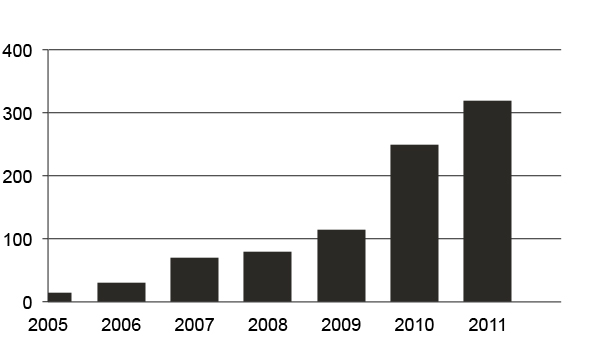
\includegraphics[height=8cm]{oh_project_evolution.jpg}
    \end{center}
    \caption{Creation of new open hardware project per year between 2005 and 2011. Graphic extracted from \emph{HOPE 2010 - How to run an open source hardware company}}
    \label{fig:oh_project_evolution}
\end{figure}


\begin{figure}[]
    \begin{center}
        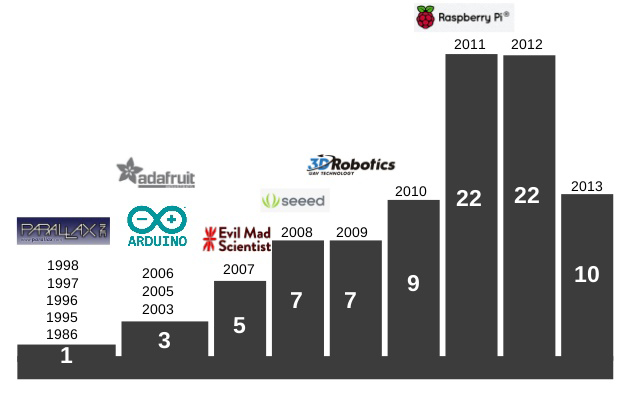
\includegraphics[height=8cm]{oh_startup_creation.jpg}
    \end{center}
    \caption{Start-up creation based on open hardware distribution}
    \label{fig:oh_startup_creation}
\end{figure}

\subsection{Famous projects} % (fold)



\subsubsection{Arduino} % (fold)

Started in 2005, the Arduino project aimed to offer an affordable and easy to use electronics board for students. Back at this time, students from the Interaction Design Institute Ivrea in Italy were using \emph{BASIC Stamp}\footnote{A BASIC Stamp module is a single-board computer that runs the Parallax PBASIC language interpreter in its microcontroller.} at a cost of \$100.

\begin{NFfigure}
    \begin{center}
        
\includegraphics[height=3cm]{arduino_logo.png}
    \caption{The Arduino logo}
    \label{fig:arduino_logo}
    \end{center}
\end{NFfigure}

To make the board, the development team had a specific, student-friendly price as their goal: \$30. \emph{It had to be the equivalent of going out to dinner at a pizza place}, Banzi said \footnote{David Kushner (26 Oct 2011). \emph{The Making of Arduino}. IEEE Spectrum.}.

A hardware thesis by Hernando Barragan\cite{barragan2004wiring} was contributed for a wiring design. After the wiring platform was complete, researchers worked to make it lighter, less expensive, and available to the open source community. The open-source model had long been used to fuel innovation for software, but not hardware. To make it work, they had to find an appropriate licensing solution that could apply to their board. After some investigation, they realized that if they simply looked at their project differently, they could use a license from Creative Commons, the nonprofit group whose agreements are normally used for cultural works such as music and writing. \emph{You could think of hardware as piece of culture you want to share with other people}, Banzi said.

Arduino is a platform for prototyping interactive objects using electronics. It consists of both hardware and software: a circuit board that can be purchased at low cost or assembled from freely-available plans; and an open-source development environment and library for writing code to control the board. Arduino comes from a philosophy of learning by doing and strives to make it easy to work directly with the medium of interactivity. It extends the principles of open source to the realm of hardware, supporting a community of people working with and extending the platform. It has been used in universities around the world and in numerous works of interactive art.\cite{mellis2007arduino}



\subsubsection{Raspberry Pi} % (fold)
\begin{row}{4}{2}
    \begin{cell}{3}
    The Raspberry Pi is a credit-card-sized single-board computer developed in the UK by the Raspberry Pi Foundation with the intention of promoting the teaching of basic computer science in schools.
    \end{cell}
    \begin{cell}{1}
    \begin{NFfigure}
    \begin{center}
        
\includegraphics[height=3cm]{raspberry_pi_logo.png}
    \end{center}
    \caption{The Raspeberry Pi logo}
    \label{fig:raspberry_pi_logo}
\end{NFfigure}
    \end{cell}
\end{row}




\begin{NFfigure}
    \begin{center}
        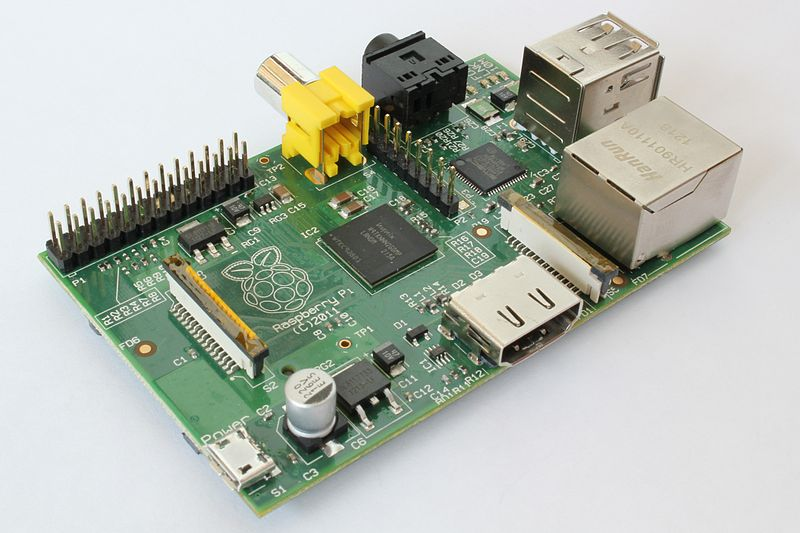
\includegraphics[height=5cm]{raspberry_pi.jpg}
    \end{center}
    \caption{The Raspeberry Pi board}
    \label{fig:raspberry_pi}
\end{NFfigure}

\subsubsection{Shapeoko} % (fold)

\begin{NFfigure}
    \begin{center}
        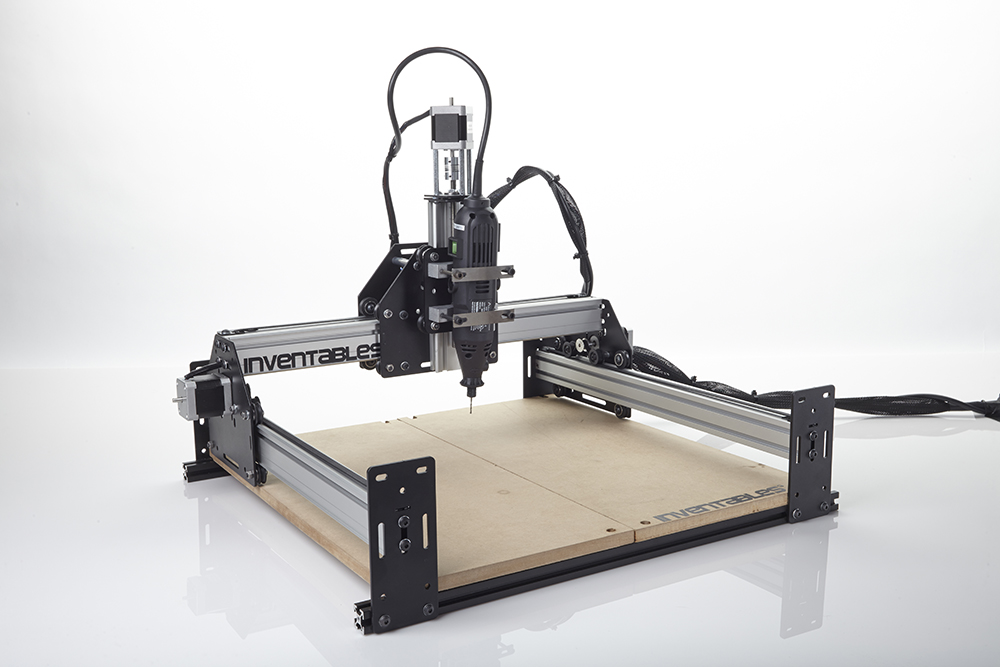
\includegraphics[height=5cm]{shapeoko_v2.jpg}
    \end{center}
    \caption{Caption here}
    \label{fig:shapeoko_v2}
\end{NFfigure}

\subsubsection{RepRap} % (fold)

The RepRap project was the first low cost 3D printer.
\begin{quotation}
RepRap takes the form of a free desktop 3D printer capable of printing plastic objects. Since many parts of RepRap are made from plastic and RepRap prints those parts, RepRap self-replicates by making a kit of itself - a kit that anyone can assemble given time and materials. It also means that - if you've got a RepRap - you can print lots of useful stuff, and you can print another RepRap for a friend...
\end{quotation}


\begin{NFfigure}
    \begin{center}
        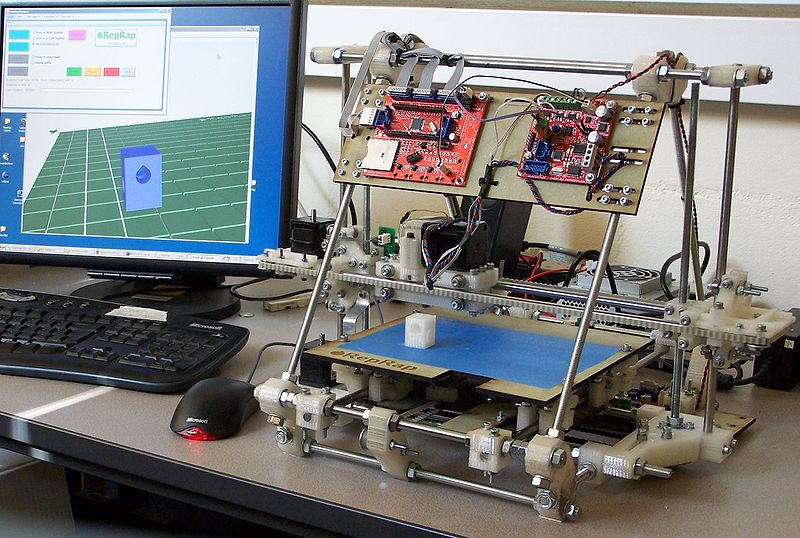
\includegraphics[height=5cm]{RepRap_v2.jpg}
    \end{center}
    \caption{Caption here}
    \label{fig:RepRap_v2}
\end{NFfigure}


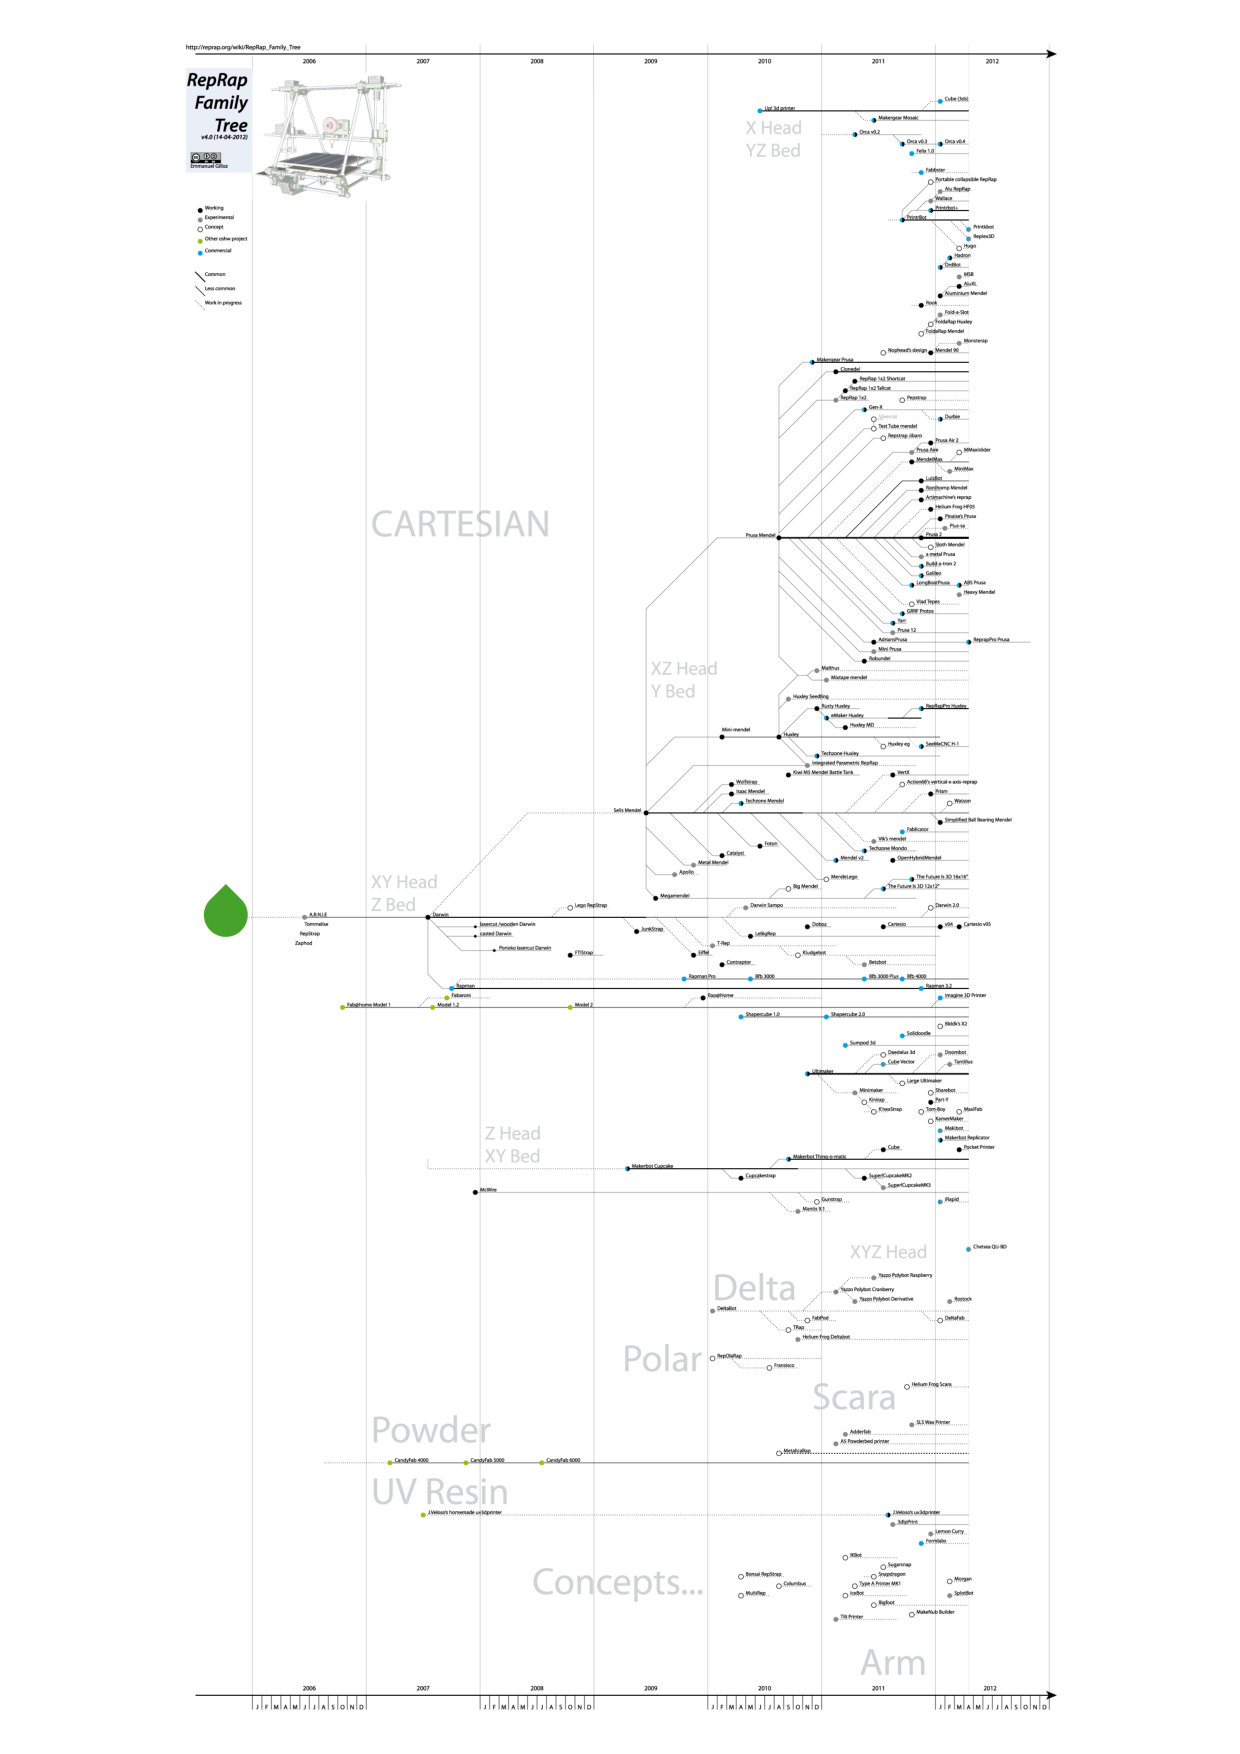
\includepdf{/Users/matthieulapeyre/Documents/phd_thesis/media/open_hardware/reprap_family_tree.pdf}

\begin{figure}[]
    \begin{center}
        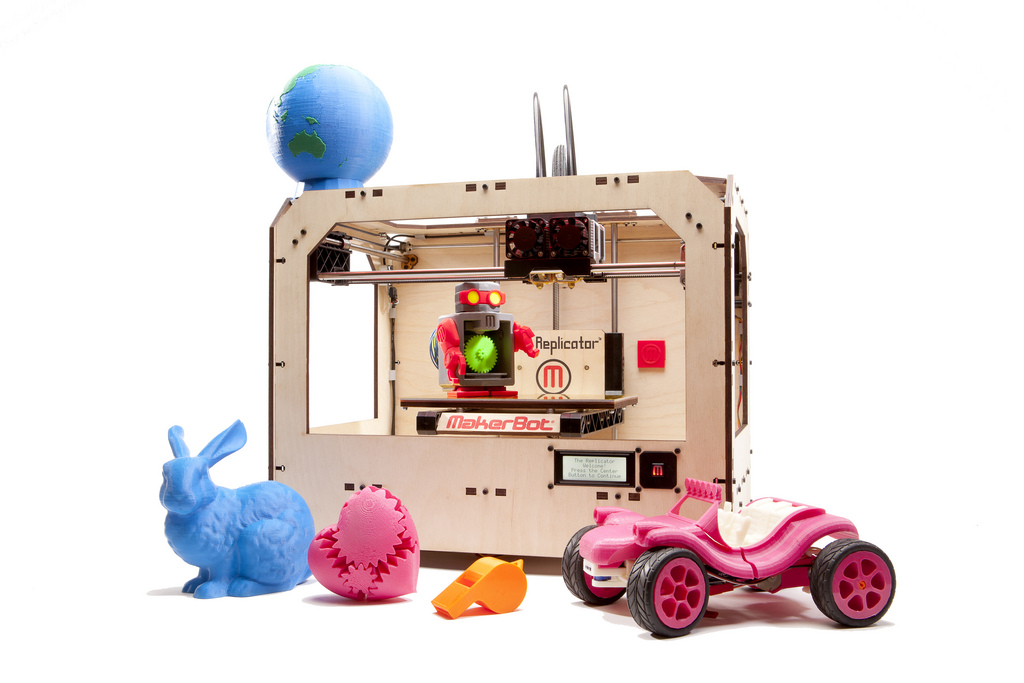
\includegraphics[height=8cm]{makerbot-replicator.jpg}
    \end{center}
    \caption{Caption here}
    \label{fig:makerbot-replicator}
\end{figure}

the ikea effect

Von Hippel, Eric (2002) "Shifting Innovation to Users via Toolkits", Management Science Vol 48, No 7, July
 Von Hippel, Eric (1986) Lead Users: A source of Novel Product Concepts. Management Science. Vol 32, No 7,
July 1986

Von Hippel, Eric (1994). " Sticky Information and the locus of problem solving: Implications for innovation."
Management Science, 40(4) 429-439

http://www.ohanda.org/


\section{Rapid prototyping} % (fold)

\paragraph{A comparison of rapid prototyping technologies (Pham 1997)}

"Prototyping is an essential part of the product development and manugacturing cycle required for assessing the forim, fit and functionality of a design before a significant investment in tooling is made. Until recently, prototypes were largerly handmade by skilled craftsmen, adding weeks or months to the product development time. Because of this, only a few design iterations could be made before tooling went into production, resulting in parts which at best were seldom optimised and at worst did not function properly.
Rapid Prototyping is a term which embraces a range of new technologies for producing accurate parts directly from CAD models in a few hours, with littel need for human intervention. This means that desigenrs have the freedom to produce physical models of theirs drawings more frequently, allowing them to check the assembly and function of the design as well as discussing downstream manufacturing issues with an easy-to-interpret, unambigous prototype. Consequently, errors are minimised and product development costs and lead times substantially reduced. It has been claimed that rapid proto can cut new product costs by up to 70\% and the time to market by 90\%."
- Rapid product development in the USA, Europe and Japan (Waterman 1994)


\subsection{Several technologies} % (fold)

\subsubsection{Stereolithography (SL)} % (fold)

This relies on a photosensitive monomer resin which forms a polymer and solidifies when exposed to ultraviolet (UV) light. Due to the absorption and scattering of the beam this reaction only takes place near the surface.

Y'en a plein dans A comparison of rapid prototyping technologies (Pham 1997)

\subsubsection{Selective laser sintering} % (fold)
SLS uses a fine powder which is heated with a CO2 laser of power in the range of 25-50W such that the surface tensions of the grains are overcome and they fuse together.Before the powder is sintered, the entire bed is headted to just below the melting point of the material in order to minimize thermal distortion and facilitate fusion to the previous layer.

\subsubsection{Filament} % (fold)




\subsection{Introduction} % (fold)

Production process by material addition.



\section{Makers \& Fablab: } % (fold)

http://alternatives.blog.lemonde.fr/2014/04/06/ces-projets-open-source-qui-changent-le-monde/



http://www.gizmag.com/disney-research-3d-printed-optics/24435/
http://www.3ders.org/articles/20131119-first-ever-3d-printed-electronics-set-to-launch-into-space-today.html
